%%	SECCION documentclass																									 %%	
%%---------------------------------------------------------------------------%%
\documentclass{report}

%%---------------------------------------------------------------------------%%
%%	SECCION usepackage																											 %%	
%%---------------------------------------------------------------------------%%
\usepackage{amsmath, amsthm}
\usepackage[spanish,activeacute]{babel}
\usepackage{caratula}
\usepackage{a4wide}
\usepackage{hyperref}
\usepackage{fancyhdr}
% \usepackage{moreverb}
\usepackage{graphicx} % Para el logo magico!
\usepackage{capt-of}
\usepackage{afterpage}
\usepackage{float}
\usepackage{amssymb}
\usepackage{amsmath}
\usepackage[latin1]{inputenc}
\usepackage{subfigure}
\usepackage[dvipsnames,usenames]{color}
\usepackage{amsfonts}
\usepackage{pdflscape}
\usepackage{booktabs}
\usepackage{colortbl}
\usepackage{tabularx}
%%---------------------------------------------------------------------------%%
%%	SECCION opciones																												 %%	
%%---------------------------------------------------------------------------%%
\parskip    = 11 pt
\headheight	= 13.1pt
\pagestyle	{fancy}
\definecolor{orange}{rgb}{1,0.5,0}

\addtolength{\headwidth}{1.0in}

\addtolength{\oddsidemargin}{-0.5in}
\addtolength{\textwidth}{1.0in}
\addtolength{\topmargin}{-0.8in}
\addtolength{\textheight}{0.7in}

%%---------------------------------------------------------------------------%%
%%	SECCION document	 %%	
%%---------------------------------------------------------------------------%%
\begin{document}
\renewcommand{\chaptername}{Parte }

%%---- Caratula -------------------------------------------------------------%%
\materia{Ingenier�a de Software I (2do cuatrimestre de 2008)}
\titulo{Trabajo Pr�ctico 0}

\integrante{Gonzalez, Emiliano}{426/06}{xjesse\_jamesx@hotmail.com}
\integrante{Gonzalez, Sergio}{481/06}{seges.ar@gmail.com}
\integrante{Mart'inez, Federico}{17/06}{federicoemartinez@gmail.com}
\integrante{Sainz-Tr�paga, Gonzalo}{454/06}{gonzalo@sainztrapaga.com.ar}
\grupo{Grupo 5}
\resumen{
}

\newcommand{\negrita}[1]{{\bf #1}}


% ----- Token list para las instrucciones ------------------------------------
\newtoks\oplist\oplist={}
% ----- Comando para que el usuario agregue operaciones del CU

\newcounter{PasoCu}
\setcounter{PasoCu}{1}

\newcommand{\op}[2]
{
\oplist=\expandafter{\the\oplist #1 & #2\\}
\stepcounter{PasoCu}
}

\definecolor{light-gray}{gray}{0.9}
\newcommand{\cu}[6]{ 
{\setlength{\arrayrulewidth}{1mm}

\begin{tabularx}{16cm}{|X|X|}
\hline
\multicolumn{2}{|>{\columncolor{Black}}l|}{\textcolor{White}{\negrita{Caso de Uso: #1}}} \\
\hline
\multicolumn{2}{|>{\columncolor{light-gray}}l|}{\negrita{Actores intervinientes: #2}} \\
\hline
\multicolumn{2}{|>{\columncolor{light-gray}}l|}{\negrita{Requerimientos relacionados: #3}} \\
\hline
\multicolumn{2}{|>{\columncolor{light-gray}}l|}{\negrita{Precondicion: #4}} \\
\hline
\multicolumn{2}{|>{\columncolor{light-gray}}l|}{\negrita{Poscondicion: #5}} \\
\hline
\multicolumn{1}{|>{\columncolor{light-gray}}X|}{\negrita{Descripcion:}} &
\multicolumn{1}{|>{\columncolor{light-gray}} X|}{\negrita{#6}} \\
\hline
\multicolumn{1}{|>{\columncolor{light-gray}}X|}{\negrita{Curso normal}} &
\multicolumn{1}{|>{\columncolor{light-gray}}X|}{\negrita{Curso alternativo}}\\
\hline
\the\oplist
\hline
\end{tabularx}

}
\newtoks\oplist\oplist={}
}

\newcounter{req}
\setcounter{req}{1}


\newcommand{\desreq}[5]{
{\setlength{\arrayrulewidth}{1mm}
\begin{tabular}{|| c | p ||}
\multicolumn{1}{|>{\columncolor{Black}}c|}{\textcolor{White}{\negrita{Requerimiento:}}} &
\multicolumn{1}{|>{\columncolor{Black}}l|}{\textcolor{White}{#1}}\\
\hline
\multicolumn{1}{|>{\columncolor{light-gray}}c|}{\negrita{Numero:}} &
\multicolumn{1}{|l|}{\thereq}\\
\hline
\multicolumn{1}{|>{\columncolor{light-gray}}c|}{\negrita{Tipo:}} &
\multicolumn{1}{|l|}{#2}\\
\hline
\multicolumn{1}{|>{\columncolor{light-gray}}c|}{\negrita{Importancia:}} &
\multicolumn{1}{|l|}{#3}\\
\hline
\multicolumn{1}{|>{\columncolor{light-gray}}c|}{\negrita{Descripci�n:}} &
\multicolumn{1}{|p{15cm}|}{#4}\\
\hline
\multicolumn{1}{|>{\columncolor{light-gray}}c|}{\negrita{Motivo:}} &
\multicolumn{1}{|p{15cm}|}{#5}\\\hline
\end{tabular}
\stepcounter{req}
}
}

% TOC, usa estilos locos
\maketitle
\pagestyle{empty}
{
\fancypagestyle{plain}
    {
    \fancyhead{}
    \fancyfoot{}
    \renewcommand{\headrulewidth}{0.0pt}
    } % clear header and footer of plain page because of ToC
\tableofcontents
}

\newpage
% arreglos los estilos para el resto del documento, y
% reseteo los numeros de pagina para que queden bien
\pagenumbering{arabic}
\fancypagestyle{plain} {
    \fancyhead[LO]{Gonzalez, Gonzalez, Mart�nez, Sainz-Tr�paga}
    \fancyhead[C]{}
    \fancyhead[RO]{P\'agina \thepage\ de \pageref{LastPage}}
    \fancyfoot{}
    \renewcommand{\headrulewidth}{0.4pt}
}
\pagestyle{plain}

\chapter{Introducci�n}

\section{Consideraciones sobre el informe}

El siguiente informe encompasa el dise�o que desarrollamos para la implementaci�n del
software de pizzer�a que fuera especificado en el Trabajo Pr�ctico 1. Nuestros objetivos
a la hora de dise�ar se enfocaron esencialmente en la flexibilidad y mantenibilidad del
software, con el objeto de que introducir cambios y correcciones en el software en
el futuro sea tan sencillo como sea posible.

En esta primera secci�n se describe brevemente el siguiente informe, as� como
su organizaci�n y contenidos y los objetivos que se plantea. En particular, este
documento est� dirigido a los desarrolladores que deber�n implementar el sistema.
Si bien no es de car�cter definitivo, el esp�ritu del documento intenta no ser
ambiguo y tener en cuenta tantas decisiones de dise�o significativas como sea
posible.

Al realizar el dise�o fue necesario en algunos casos introducir modificaciones o mejoras
a lo anteriormente especificado. Dichos cambios se evaluaron y fueron juzgados necesarios
por las ventajas que representan en varios planos, pero particularmente en la extensibilidad
y flexibilidad del sistema para tolerar cambios futuros en su modo de operaci�n. La segunda
secci�n del informe describe los cambios realizados as� como la justificaci�n de los mismos
y el impacto que tienen en el dise�o.

En tercer lugar se presenta la descripci�n del dise�o propiamente dicha. Como se adopt�
un acercamiento por componentes, se describe inicialmente esta divisi�n en componentes,
sus ventajas y limitaciones as� como la raz�n de utilizar esta modalidad. Enseguida se
presenta el dise�o de cada componente, as� como las relaciones que existen entre los
objetos de los mismos. Por �ltimo, se utiliza la herramienta de diagramas de secuencia
para modelar las comunicaciones entre los objetos (dentro de un mismo componente, o
entre varios de ellos). En los casos en que fue considerado necesario, se adjunta adem�s
el pseudoc�digo de algunos algoritmos de inter�s.

\section{Convenciones de notaci�n}

A lo largo de este documento se utilizan las siguientes convenciones:
\begin{itemize}
\item \textbf{DIP}: \textit{Dependency Inversion Principle}
\item \textbf{OCP}: \textit{Open/Closed Principle}
\item \textbf{SRP}: \textit{Single Responsibility Principle}
\item \textbf{LSP}: \textit{Liskov Substitution Principle}
\item \textbf{ISP}: \textit{Interface Segregation Principle}
\end{itemize}

En los diagramas de secuencia muchas veces la sintaxis no se ajusta exactamente a la descripta
en clase (por ejemplo, en el caso de las variables locales a un \textit{loop}). Esto se debe en parte
a limitaciones de la herramienta utilizada para realizar los diagramas, y en parte a que la sintaxis
propuesta no es UML y por lo tanto no est� soportada.

\chapter{Descripci�n General}
\textcolor{Blue}{Esta secci�n busca describir los factores generales que afectan al producto y sus requerimientos. No se detallan aqu� los requerimientos espec�ficos, pero provee un conocimiento b�sico general para dichos requerimientos.}

\section{Perspectiva del producto}
\textcolor{Blue}{Esta secci�n encuadra el producto en la perspectiva con otros productos relacionados. Si el producto es independiente y totalmente autocontenido, dicha situaci�n deber�a explicitarse aqu�.}

\section{Funciones principales del producto} 
\textcolor{Blue}{Esta secci�n deber�a proveer un resumen de las funciones principales que el producto debe realizar. }

\section{Caracter�sticas de los usuarios}
\textcolor{Blue}{Esta secci�n deber�a describir las caracter�sticas generales de los usuarios para los que est� pensado el producto.} 

\section{Restricciones}
\textcolor{Blue}{Esta secci�n deber�a proveer una descripci�n general de cualquier cuesti�n que limite las opciones del desarrollador (ej, regulaciones, limitaciones de hardware, requerimientos sobre lenguajes de alto nivel, etc.)}

\section{Supuestos y dependencias}
\textcolor{Blue}{Esta secci�n deber�a enumerar cada uno de los factores que afectan los requerimientos declarados en el documento. Estos factores no son restricciones de dise�o del software, sino m�s bien representan cuestiones cuyo cambio puede afectar los requerimientos.}

\chapter{Requerimientos espec�ficos}
%{\color{Blue} Esta secci�n deber�a contener todos los requerimientos en un nivel de detalle suficiente para permitir:
%
%*	a los dise�adores de software: realizar un dise�o que satisfaga los requerimientos
%
%*	a los analistas de pruebas: verificar que el software satisface los requerimientos
%
%A trav�s de esta secci�n, cada requerimiento declarado deber�a ser perceptible por usuarios, operadores y otros sistemas externos. Estos requerimientos deber�an incluir, al menos,  una descripci�n de cada entrada (est�mulo) del software , de cada salida (respuesta) del software, y de todas las funciones que debe realizar el software en respuesta de una entrada o como soporte a una salida.
%Esta secci�n es la m�s importante del presente documento.}
%
%{\color{ForestGreen}CdC: En esta secci�n se espera que se describan los requerimientos espec�ficos utilizando las distintas t�cnicas vistas en la materia. Se espera encontrar:
%
%$\wp$	Diagrama de contexto
%
%$\wp$	Se espera al menos que est�n modelados los fen�menos esenciales identificados.
%
%$\wp$	Modelo de Objetivos
%
%$\hbar$	Se espera al menos que est�n bien refinados los objetivos principales  y los requerimientos esenciales (ver secci�n Matriz de requerimientos) para la m�quina a construir, y obviamente todo el grafo para cubrir el camino entre ellos. La parte explicitada del diagrama debe ser completa y correcta. 
%
%\hspace{3cm} * Todos los objetivos en el camino hacia los requerimientos esenciales deben ser refinados (al menos para explicitar ese camino).
%
%\hspace{3cm} * Puede ser que alg�n objetivo no se refine porque no sea relevante en el camino a requerimientos esenciales; pero todo objetivo refinado debe incluir a todos los subobjetivos inmediatos.
%
%$\hbar$	Enumeraci�n de todos los requerimientos detectados, con una breve descripci�n de cada uno, e identificaci�n de si se trata de un requerimiento funcional o no funcional. Adem�s, cada requerimiento deber� clasificarse como esencial, importante o deseable (debe tener coherencia con el Modelo de Objetivos). En esta clasificaci�n se entiende por:
%
%$\diamond$	requerimientos esenciales: aquellos requerimientos que caracterizan la esencia del software a  construir. Sin estos requerimientos, el software ya dejar�a de ser lo que se espera.
%
%$\diamond$	requerimientos importantes: aquellos requerimientos que son necesarios para que el software funcione de acuerdo a lo esperado, pero no son esenciales. Su incumplimiento provocar�a la no aceptaci�n del software.
%
%$\diamond$	requerimientos deseables: aquellos que representan alguna funcionalidad opcional, su cumplimiento es deseado por el cliente, pero su incumplimiento no provocar�a el rechazo del software.
%
%$\wp$	Casos de Uso
%
%$\hbar$	Actores
%
%$\hbar$	Diagramas.
%
%$\hbar$	Descripci�n de cada caso de uso
%
%$\wp$	Operaciones relevantes
%
%$\hbar$	Describir operaciones relevantes ( si lo necesitan) usando una combinaci�n de t�cnicas de documentaci�n de casos de uso y/o OCL  y/o lenguaje natural.
%
%$\wp$	Diagramas de Actividad
%
%$\hbar$	Diagramas de actividad que consideren necesarios. En cada caso se debe indicar a que requerimientos y/o casos de uso u otro artefacto hace referencia. 
%
%$\wp$	M�quinas de estado finito
%
%$\hbar$	M�quinas de estado finito que consideren necesarias. En cada caso se debe indicar a que requerimientos y/o casos de uso se hace referencia.
% 
%$\wp$	Modelo Conceptual
%$\hbar$	Diagrama
%$\hbar$	Diccionario de datos
%$\hbar$	Restricciones al MC (utilizando OCL)
%
%$\wp$	Prototipos de Pantalla
%$\hbar$	Prototipos de las pantallas que se consideren importantes para validar. 
%$\hbar$	Se espera que permitan dar una idea de la informaci�n input y ouptut que deber�a mostrarse. No es necesario poner �nfasis en el aspecto est�tico definitivo de la interfaz usuario, s�lo que permita comunicar la pantalla desde un punto de vista de la funcionalidad y la interacci�n posible del usuario.
% 
% 	CdC: La organizaci�n de los Requerimientos Espec�ficos es una parte importante de la evaluaci�n. Deben presentarlo de la manera que consideren m�s apropiada de manera de poder comunicar las ideas.
% 	 
% 	CdC: No es obligatorio utilizar todas las t�cnicas mencionadas, queda a criterio de cada grupo (y es parte de la evaluaci�n) la elecci�n de la t�cnica m�s apropiada para cada aspecto que quieran modelar, as� como la decisi�n de los aspectos modelados.}
\begin{landscape}
\section{Diagrama de contexto}
\begin{figure}[H]
\centering
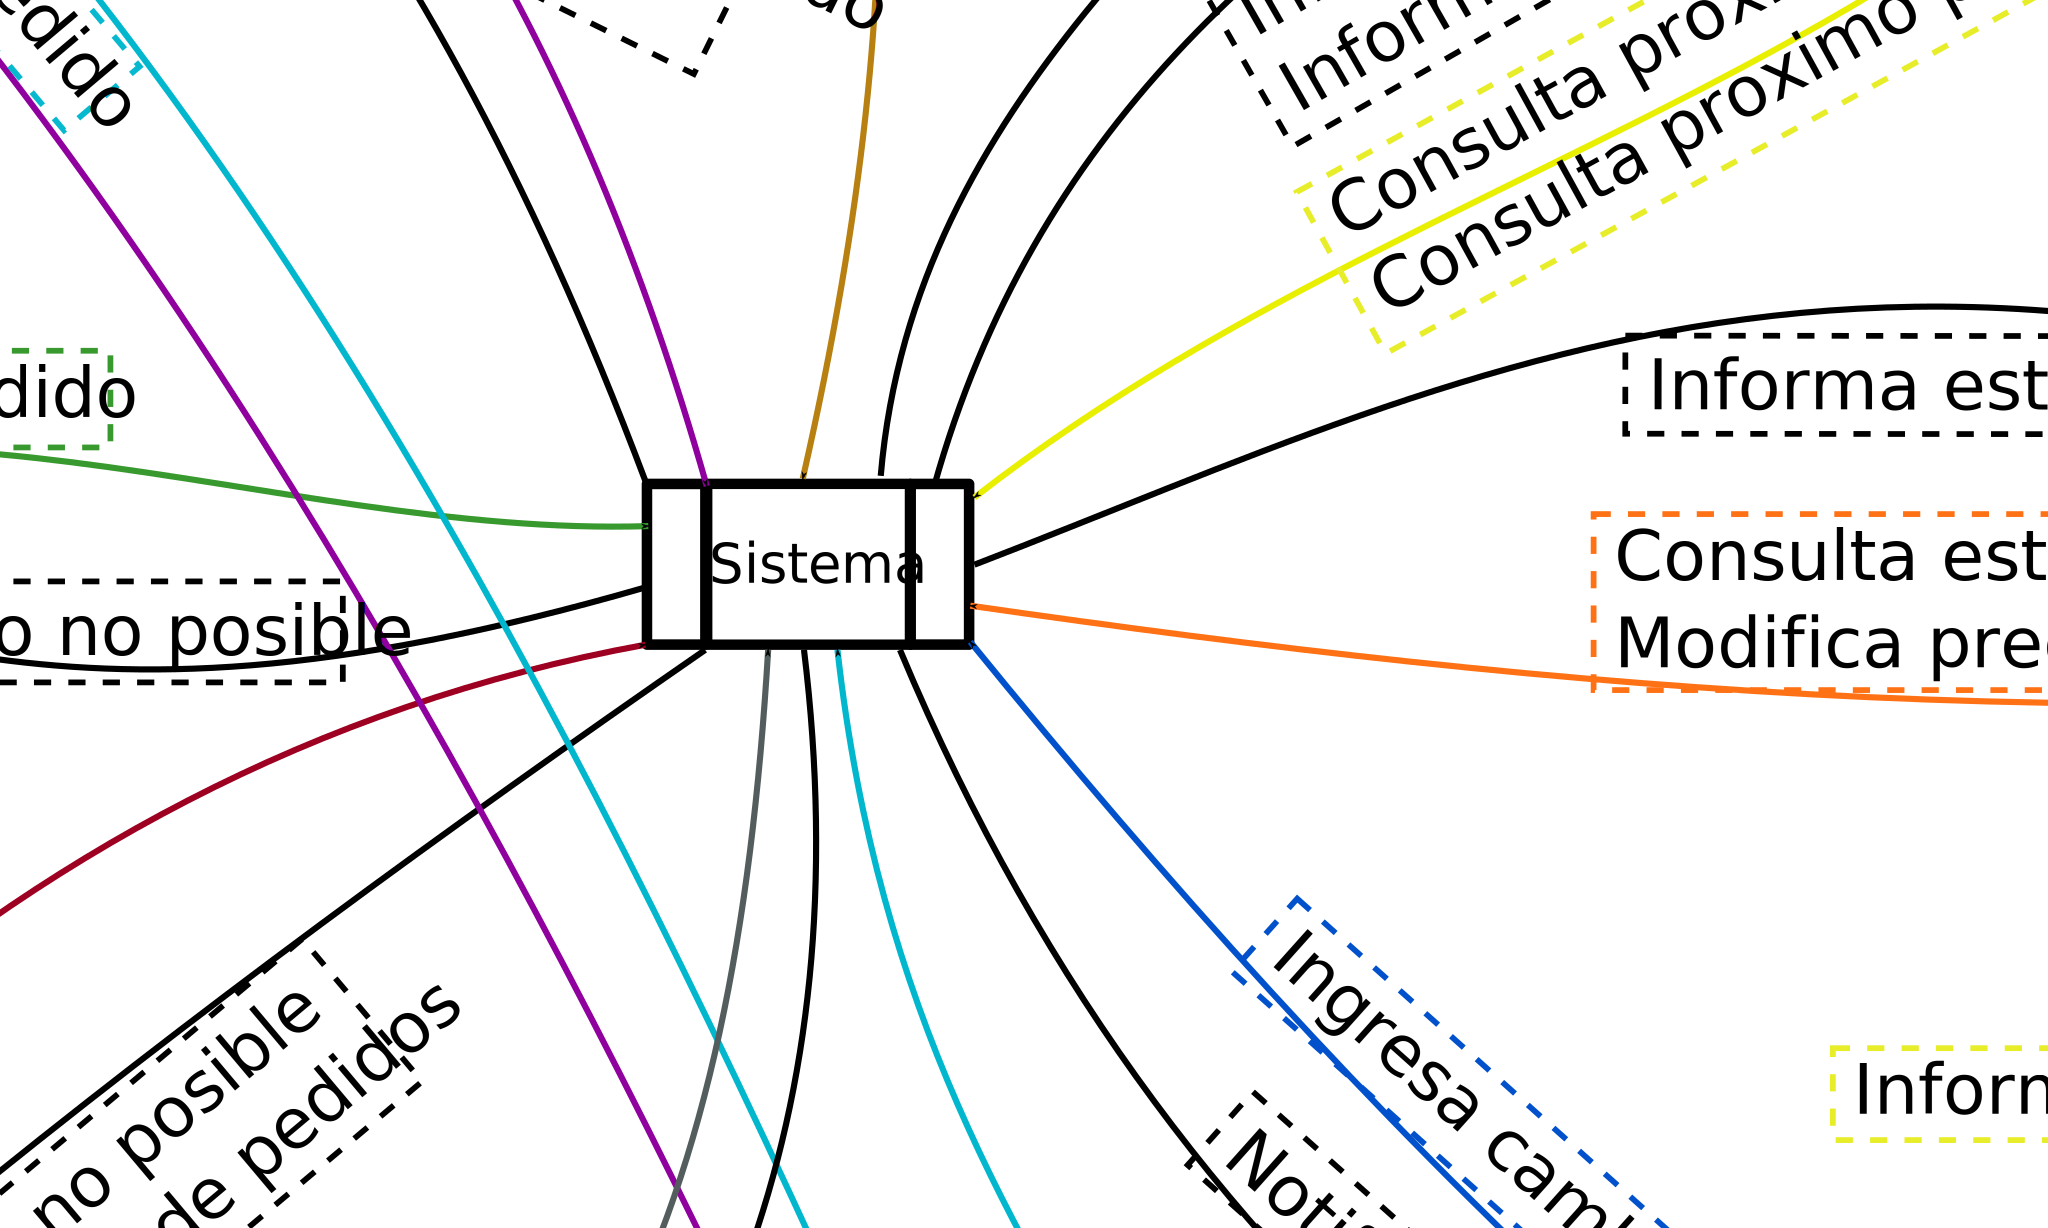
\includegraphics[height=16cm]{ContextoNormal.png}
\end{figure}
\begin{figure}[H]
\centering
\includegraphics[height=16cm]{ContextoNormalSimplificado.png}
\end{figure}
\begin{figure}[H]
\centering
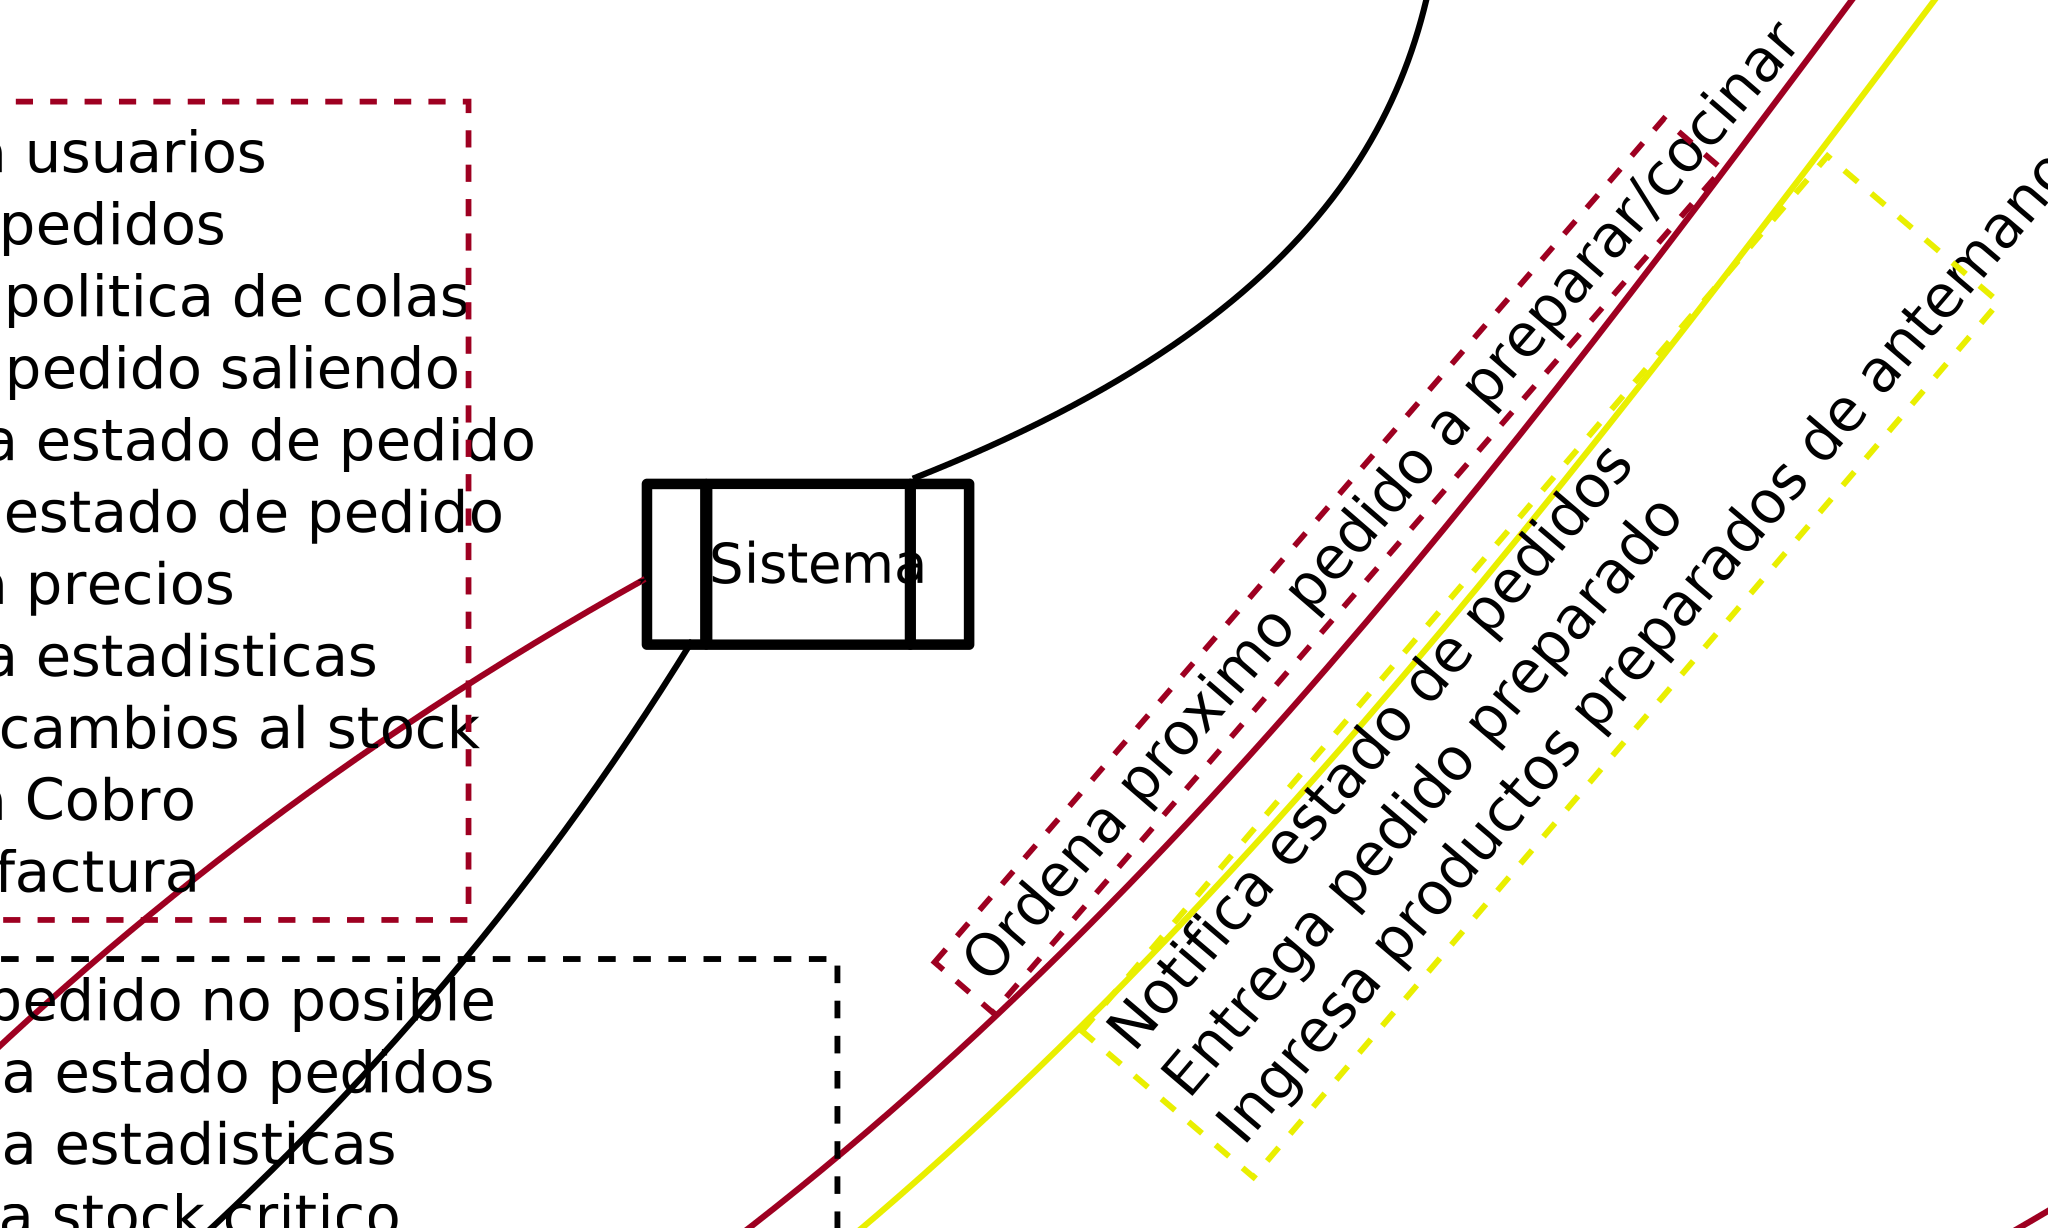
\includegraphics[height=16cm]{ContextoContingencia.png}
\end{figure}
\end{landscape}

\begin{landscape}
\section{Modelo de objetivos}
\subsection{Diagrama de objetivos}
Dado el tama�o del diagrama y para facilitar su lectura decidimos fragmentar el mismo. Las partes se encuentran a continuacion:

\begin{figure}[H]
\centering
\includegraphics[height=14.5cm]{DiagramaObjetivos4.png}
\end{figure}
\begin{figure}[H]
\centering
\includegraphics[height=14.5cm]{DiagramaObjetivos3.png}
\end{figure}
\begin{figure}[H]
\centering
\includegraphics[height=14cm]{DiagramaObjetivos2.png}
\end{figure}
\begin{figure}[H]
\centering
\includegraphics[height=14.5cm]{DiagramaObjetivos1.png}
\end{figure}
\end{landscape}

\subsection{Descripci�n de los requerimientos}

\desreq{Poder hacer pedido desde pagina web}{Funcional}{Importante}{El usuario tiene que poder ingresar un pedido desde la p�gina web de la pizzer�a}{El cliente debe poder hacer pedidos via web y asi ampliar las formas de hacer pedidos}

\desreq{Poder identificar al usuario cuando se loguea}{Funcional}{Importante}{Es necesario poder identificar al usuario que quiere utilizar algun servicio de la pizzeria via web}{El cliente debe poder hacer pedidos via web y asi ampliar las formas de hacer pedidos}

\desreq{Mantener base de datos de clientes actualizada}
{Funcional}
{Importante}
{Una base de datos actualizada es necesaria para poder tener informaci�n de los usuarios y permitirles realizar pedidos remotos}
{Mantener base de datos de clientes}

\desreq{Lograr que el cliente se pueda registrar en la base de datos}{Funcional}{Importante}{Debe poder registrarse nuevos usuarios en la base de datos del sistema}{Mantener base de datos de clientes}

\desreq{Identificar al cliente por su n�mero de celular}
{Funcional}
{Importante}
{Asi como para el caso web, para poder hacer un
pedido via SMS es necesario poder identificar el n�mero del celular que 
env�a el mensaje con el cliente registrado}
{Lograr que el cliente haga pedidos via SMS}

\desreq{Interactuar con servicio externo de cobros con tarjeta de credito}
{Funcional}
{Importante}
{El sistema debe ser capaz de interactuar con algun servicio similar a paypal}
{El cliente puede pagar pedidos con tarjeta desde la web}

\desreq{Poder identificar a un pedido de forma unica}
{Funcional}
{Importante}
{Debe ser posible referenciar a un pedido ingresado al sistema de forma univoca}
{Que el usuario pueda consultar el estado de sus pedidos via web}

\desreq{Estimar tiempos de preparacion de pedidos de forma dinamica}
{No funcional} %TODO:dice como tiene q hacerse, verificar
{Deseable}
{En vez de ingresar a mano el tiempo de preparaci�n de pedidos, una alternativa es ir estimando dinamicamente los tiempos
de preparaci�n, de este modo se puede adaptar la estimaci�n seg�n la cantidad de pedidos que tenga que atender la cocina}
{Permitir tener una estimaci�n para los productos individuales}

\desreq{Calcular tiempo total de cocci�n de un pedido en base a estimaciones individuales}
{Funcional} %TODO: no se si es func o no
{Importante} %todo: no se tampoco
{Los tiempos individuales para los productos deben usarse para poder estimar el tiempo de un pedido teniendo en cuenta la cola
de producci�n, la politica de asignaci�n, etc}
{Se desea estimar el tiempo de preparaci�n de los pedidos}

\desreq{Poder modifiar la cola de pedidos}
{Funcional}
{Deseable}
{El encargado de pedidos debera tener una interfaz que le permita modificar la politica de administracion de cola}
{Se pide que el sistema sea flexible para incorporar nuevas politicas de cola}

\desreq{Aplicar politica de cola prestablecido}
{Funcional}
{Esencial}
{El sistema debera mostrar que pedido debe ingresar al horno en cada momento}
{Se pide explicitamente que el software debe indicar que pedido cocinar, ademas sirve para lograr un orden eficiente de los pedidos}

%TODO:no entiendo la diferencia entre aplicar y mostrar prox
%FIXME: cual es el q se relaciona derecho con el horno?
\desreq{Informar proximo pedido a preparar}
{Funcional}
{Esencial}
{El sistema debera informar a los maestros que deben preparar en cada momento}
{Se pide explicitamente, ademas es necesario para lograr un orden eficiente en los pedidos}

\desreq{Poder modificar el estado de los pedidos a lo largo de su ciclo de vida}
{Funcional}
{Esencial}
{El sistema debe permitir que los distintos agentes que modifican el estado de un pedido puedan registrar ese
cambio de estado, por ejemplo el maestro debe poder informar que un pedido esta preparado}
{Se pide explicitamente poder conocer el estado de un pedido, ademas sirve para fines estadisticos, asi como tambi�n para brindar informaci�n a los clientes}

\desreq{El sistema debe poder funcionar en caso de contingencia desde el puesto del encargado de pedidos}
{Funcional}
{Deseable}
{En caso de caida de los otros puestos de trabajo, el sistema debe permitir que el encargado de pedidos ingrese, y tenga acceso a, la informaci�n necesaria para el funcionamiento del software}
{Es una alternativa deseable propuesta por los clientes, permite un sistema mas tolerante a fallos}

\desreq{Es posible ingresar datos ocurridos fuera del sistema para su registro y facturaci�n}
{Funcional}
{Deseable}
{Luego de una caida del sistema deber�a ser posible lograr cargar manualmente los pedidos que ocurrieron durante el tiempo en el que el sistema estuvo caido}
{Lograr un software mas tolerante a fallos}

\desreq{Al cancelar un pedido se elimina el stock si se cancela despues de cocinar}
{Funcional}
{Importante}
{Si un pedido se cancela luego de haber sido cocinado, el stock no debe volver a reestablecerse ya que no puede ser reutilizado}
{Poder controlar las cancelaciones con el fin de conocer plenamente el estado de los pedidos}

\desreq{Al cancelar un pedido se guarda el pedido preparado si no estaba cocinado}
{Funcional}
{Deseable} % o importante?
{En el caso de que la cancelaci�n se haga luego de ser preparado, pero aun no cocinado, el sistema puede registrar que los productos del pedido estan ya preparados a fin de que puedan utilizarse en algun pedido futuro}
{Poder controlar las cancelaciones, mejorar la eficiencia de la cocina}

\desreq{Se restaura el stock si el pedido no estaba preparado, al cancelarlo}
{Funcional}
{Importante}
{Si se cancela antes de preparlo, las materias primas que no se usaron deben volver al stock a fin de que puedan ser usadas para preparar un nuevo pedido}
{Poder controlar las cancelaciones, mejorar la eficiencia de la cocina}

\desreq{Se alerta al responsable en caso de que el stock de un producto sea critico}
{Funcional}
{Esencial}
{Cuando el stock de un producto queda por debajo de un limite preestablecido se debe generar algun mensaje para el responsable del stock a fin de notificar de esta situaci�n}
{Es una funcionalidad pedida explicitamente por el cliene, ayuda a mantener un stock apropiado de los distintos productos}

\desreq{Disponer de ABM de stock}
{Funcional}
{Importante}
{El sistema debe permitir que las altas, bajas y modificaciones de productos se registren en el sistema, para de esta manera controlar el stock de las materias primas y bebidas}
{Mantener un stock apropiado de los productos}

\desreq{La notificaci�n de pedido preparado de antemano se registra}
{Funcional}
{Deseable}
{El software podr�a permitir ingresar pedidos preparados de antemano, quedando notificado que los productos ya estan preparados para ser usado en caso de que un furuto pedido los necesite}
{Permite mantener actualizado el stock ya que las materias primas de los productos preparados de antemano deben darse de baja del stock}

\desreq{Al ingrear pedido se actualiza el stock}
{Funcional}
{Importante}
{El sistema decrementar� el stock de materias primas o bebidas necesarias para un pedido al momento en que este ingresa al sistema}
{Permite que el ingreso de pedidos modifique el stock consistentemente y de esta manera tener un stock actualizado}

\desreq{Todos los pedidos pueden registrarse en el sistema}
{Funcional}
{Esencial}
{Los pedidos realizados pueden ingresarse al sistema y este los registra}
{Poder controlar el stock y conocer el estado de los pedidos}

\desreq{Operaciones de ingreso de pedido y baja de stock son atomicas}
{No funcional} %TODO: no se
{Importante}
{Al momento de ingresar un pedido deberia ser posible hacer un lockeo de los productos necesarios, de modo que al momento de confirmar el mismo los recursos a utilizar esten efectivamente disponible}
{Evitar tomar pedidos si no se dispone de los recursos para satisfacerlos}

\desreq{Rechazar ingreso de pedido si los recursos son insuficientes}
{Funcional}
{Esencial}
{Si cuando se realiza un pedido no se dispone de los recursos necesarios para completarlo, el mismo no debe ingresar al sistema y se debe notificar a quien este intentando realizar el pedido de la situaci�n}
{Evitar tomar pedidos si no se dispone de los recursos para satisfacerlo}

\desreq{Disponer de ABM de productos}
{Funcional}
{Importante}
{Se debe proveer de una interfaz para registrar nuevos productos (por ejemplo nuevas variedades de pizza) al men� asi como tambi�n modificar precios de productos ya registrados o sacarlos del men�. Por otro lado, este ABM sirve para registrar la cantidad de materias primas que utiliza un producto}
{Conocer la cantidad de materia prima que usa un producto a fin de poder evitar tomar pedidos insatisfacibles, poder modificar lista de precios}

\desreq{Mantener estadisticas sobre productos gestionados}
{Funcional}
{Escencial} %TODO: mmmmmmm
{El sistema debe ser capaz de retener la informaci�n estadistica sobre los pedidos asi como tambi�n calcular los diferentes indicadores estadisticos descriptos en \textcolor{Peach}{Describir esto en algun lado}}%FIXME: completar esto
{Se pide de forma explicita tener informaci�n estadistica sobre el funcionamiento de la pizzeria, los pedidos, etc}

\desreq{Lograr que el usuario pueda ingresar comentarios sobre el servicio}
{Funional}
{Deseable}
{Como aporte original proponemos que el usuario pueda ingresar comentarios sobre el servicio, luego de recibir un pedido. El sistema debe ser capaz de registrar esos comentarios}
{Lograr informaci�n estadistica}

\desreq{Es posible comunicarse con el sistema de facturaci�n}
{Funcional}
{Esencial}
{El software debe ser capaz de interactuar con el sistema de facturaci�n para facturar el pago de los pedidos, asi como para poder realizar pagos con tarjeta}
{Se debe automatizar la facturaci�n y la pizzer�a ya cuenta con un software de facturaci�n}

\section{Casos de uso}
\subsection{Diagrama}
\begin{figure}[H]
\centering
\includegraphics[height=15.5cm]{casosdeuso.png}
\end{figure}
\subsection{Descripci�n de los casos de uso}
%%%%%%%%%%%%%%%%%%%%%%%%%%%%%%%%%%%%%%%%%%
% plantilla para casos de uso %%%%%%%%%%%%
%%%%%%%%%%%%%%%%%%%%%%%%%%%%%%%%%%%%%%%%%%
%\op{agrego una operacion en contexto normal}{y ahora su contexto de excepcion}
%\op{agrego otra}{lo malo es q no se numeran solas}
%\cu{nombre del caso de uso}{actor relacionado}{requerimiento}{pre}{pos}
%\oplist={} vacio la lista para otro caso de uso
%\cu{hola}{colo}{trolo}{fonolo}{rqqq}
%

%LOGUEANDO USUARIO
\op{1. El cliente ingresa su nombre de cliente en el campo correspondiente}{}
\op{2. El cliente ingresa su contrase�a en el campo correspondiente}{}
\op{3. El cliente presiona el boton de ingresar}{}
\op{4. Si los datos ingresados son validos, cliente autentificado}{4. Los datos no son validos, se muestra al cliente mensaje informativo y se le permite re ingresar los datos}
\op{5. Fin CU}{}

\cu{Logueando cliente}{Usuario}{1,2}{TRUE}{Usuario logueado}{Autentificaci�n de un cliente web}

% Haciendo pedido via web
\op{1. Usuario selecciona de una lista los productos que desea y su cantidad}{}
\op{2. El cliente presiona el boton de enviar pedido}{}
\op{3. El sistema intenta ingresar el pedido}{}
\op{4. Si el pedido es posible, se informa al cliente}{4. Si el pedido no
era posible de tomar, se muestra mensaje de error al cliente indicando que productos no estan disponibles}
\op{5. Se pregunta al cliente si desea pagar con tarjeta de credito o pagar en efectivo al delivery}{}
\op{6. Si el cliente desea pagar con tarjeta se extiende con el caso de uso Pagando pedido via web}{}
\op{7. Si se paga con tarjeta y el pago fue posible, el pedido queda registrado}{}
\op{8. Se brinda al cliente un id de pedido para poder luego consultar el estado del pedido}{}
%TODO: averiguar si la notacion de extender es la que se usa aca
\op{9. Fin CU}{}

\cu{Realizando pedido via web}{Usuario}{1}{Usuario logueado}{Pedido registrado}{Ingreso de un pedido al sistema desde la pagina web}

% Pagando pedido web
%TODO: que lo complete alguien que sepa como corno se hace un pago con tarjeta via web

%Cancelando pedido
\op{1. El cliente informa al encargado de pedido su nombre o nombre de cliente y el id de pedido, o el cliente informa al mozo que desea cancelar un pedido y el mozo informa al encargado de pedidos el deseo de la mesa de cancelar el pedido}{}
\op{2. El encargado ingresa el nombre proporcionado por el cliente y el id de pedido o revisa los pedidos de la mesa}{}
\op{3. Una vez seleccionado el pedido por el encargado, presiona el boton de cancelar pedido y el pedido queda cancelado}{3. Si los datos no corresponden con ningun pedido, el sistema muestra un cartel de error, y el encargado debe informar de la situaci�n al cliete para que verifique los datos}
\op{4. Fin CU}{}

\cu{Cancelando pedido}{Encargado de pedido}{$\infty$}{TRUE}{Pedido cancelado}{Cancelaci�n de un pedido} %TODO: deberia ser un requerimiento poder cancelar pedido
%FIXME: deberia haber precondicion?

%Realizando pedido via SMS
\op{1. El cliente escribe codigos que identifican a productos (por ejemplo: Muzza podria ser un codigo para pedir una pizza de muzzarela) asi como la cantidad (por ejemplo: Muzza 2 Napo 1, podria ser dos muzzarelas y una napolitana)}{}
\op{2. El cliente envia el mensaje a la pizzer�a}{}
\op{3. El sistema revisa si el n�mero desde donde proviene el mensaje esta registrado con alg�n cliente, si no es asi el pedido no se ingresa, fin CU}{3. Si el n�mero esta registrado pero el mensaje no corresponde con ning�n c�digo se notifica al cliente que el c�digo no es v�lido}
\op{4. El sistema revisa si es posible tomar el pedido, si es posible se ingresa el pedido, se envia al usuario un mensaje 
notificandole que su pedido esta ingresado, el importe total y el codigo de pedido para realizar consultas sobre el mismo}{3. Si no era posible se envia un mensaje indicandole que producto no estaba disponible}
\op{5. Fin CU}{}
\cu{Realizando pedido via sms}{Cliente}{$\infty$}{TRUE}{Pedido ingresado}{Ingreso de un pedido a traves de mensaje de texto}

%Ingresando feedback
\op{1. El cliente ingresa a la p�gina web de la pizzer�a}{}
\op{2. Ingresa al apartado de feedback}{}
\op{3. Ingresa el n�mero de pedido sobre el que va a emitir feedback}{}
\op{4. El sistema verifica que el n�mero de pedido corresponda con un pedido enviado por delivery}{}
\op{5. Si el n�mero era valido, se muestra un formulario al usuario para que envia sus opini�n}{5. Si el n�mero no coincide se envia un mensaje de error al usuario}
\op{6. Fin CU}{}
\cu{Ingresando feedback}{Cliente}{28}{TRUE}{Comentario ingresado}{Permite que el usuario envie al sistema su opini�n sobre un pedido recibido por delivery}

%Consultando estado de pedido
\op{1. Si el agente que desea consultar estado es el encargado de pedidos ir a 6}{}
\op{2. El cliente selecciona consultar estado de pedido}{}
\op{3. El cliente ingresa el n�mero del pedido cuyo estado quiere conocer}{}
\op{4. El sistema verifica que el n�mero de pedido corresponda a un pedido del usuario}{}
\op{5. Si es asi se muestra el estado del pedido, ir a fin CU}{5. Si no es asi se muestra un mensaje de error, pedir que ingrese de nuevo el n�mero de pedido}
\op{6.El encargado de pedidos ingresa el numero de pedido a consultar}{}
\op{7. Se verifica que el n�mero de pedido sea correcto, si es asi se muestra el estado y demas informaci�n del pedido}{7. Si no es asi se notifica con un mensaje de error}
\op{5. Fin CU}{}
\cu{Consultando estado de pedido}{Cliente, encargado de pedidos}{$\infty$}{Si el agente es un cliente entonces tiene que estar logueado}{Se muestra el estado del pedido}{Permite ver en que estado se encuentra un pedido en un momento dado}

%ingresando pedidos diferidos
\op{1. El encargado de pedidos selecciona ingresar pedido diferido}{}
\op{2. El sistema muestra la pantalla para el ingreso del pedido}{}
\op{3. El encargado ingresa los datos que conoce sobre el pedido (por ejemplo: cantidad de empanadas, pizzas, estado actual del pedido)}{}
\op{4. El encargado presiona ingresar pedido}{}
\op{5. El pedido queda ingresado}{}
\op{6. Fin CU}{}
%FIXME: ojo con este cu porque nos puede traer dolor de pelotas en el diagrama de conceptos, notar que algunos atributos que posiblemente tenga la clase pedido, este tipo de pedidos no los va a tener.

\cu{Ingresando pedido diferido}{Encargado de pedidos}{15}{}{El pedido diferido queda registrado}{Permite ingresar un pedido que no pudo ser ingresado al sistema cuando se origin�, por ejemplo porque el sistema estaba caido}

%ingresando productos de antemano
\op{1. El maestro informa al encargado de pedidos que preparo cierta cantidad de alg�n/os producto (Por ejemplo: tres empanadas de carne)}{}
\op{2. El encargado de pedidos selecciona ingresra producto de antemano en el sistema}{}
\op{3. Busca el/los producto/s que quiere ingresar y la cantidad}{}
\op{4. Presiona ingresar}{}
\op{5. El producto preparado queda registrado}{}
\op{6. Fin CU}{}

\cu{Ingreando producto de antemano}{Encargado de pedidos}{21}{El producto a ingresar tiene que ser un producto valido}{El producto preparado queda registrado}{Permite registrar productos ya preparados y que se pueden usar para futuros pedidos, sin tener que ser armados}

%estableciendo politica de cola
\op{1. El encargado de pedidos selecciona establecer politica de cola}{}
\op{2. Luego escoge uno de los hornos}{}
\op{3. El sistema lista las politicas disponibles}{}
\op{4. El encargado selecciona la que desea aplicar}{}
\op{5. Luego ingresa aceptar}{}
\op{6. La politica de coloa queda establecida}{}
\op{7. Fin CU}{} %FIXME: en que momento se aplica la modificaci�n? el cambio de politica puede dejar chingadas algunas cosas

\cu{Estableciendo politica de cola}{Encargado de pedidos}{10,11}{}{Politica de cola establecida}{Permite modificar la politica de cola de pedidos de los hornos}


%registrando pedido
\op{1. El encargado de pedidos atiende una llamada a la pizzer�a}{}
\op{2. Ingresa el n�mero del cliente que realiza la llamada}{} %TODO: se identifica por numero, nombre, DNI o q cosa?
\op{3. Si el cliente no tiene n�mero de cliente informa que tiene que registrarse, ir a fin CU}{} %FIXME: por esto registrar pedido deberia estar extendido por registrando usuario
\op{4. Si el n�mero de cliente era valido le pide el pedido}{4. Si no, le vuelve a pedir el n�mero}
\op{5. El encargado selecciona ingresar pedido}{}
\op{6. Selecciona los productos con las cantidades que el cliente solicita}{}
\op{7. Presiona aceptar}{}
\op{8. Si el pedido no se puede satisfacer, el sistema mostara un mensaje de error informando que productos no estan disponibles. El encargado notifica al cliente de la situaci�n y se vuelve a 6}{}
\op{8. El sistema notifica el total y el codigo de pedido}{}
\op{9. El encargado da esa informaci�n al cliente}{}
\op{10. Fin CU}{}

\cu{Registrando pedido}{Encargado de pedidos}{23}{}{Pedido ingresado}{Permite que el encargado de pedidos ingrese los pedidos realizados por clientes via telefono}

%ingresando pedido de mesa
\op{1. El cliente informa al mozo lo que quiere pedir}{}
\op{2. El mozo marca en su PDA los productos que el cliente pide con sus cantidades}{}
\op{3. Cuando el cliente inform� todo el pedido, el mozo selecciona ingresar pedido}{}
\op{4. Si el pedido se puede tomar, al mozo se le informa el n�mero de pedido}{4. Si no se puede tomar el pedido, se informa al mozo que partes del pedido no estan disponibles, el mozo informa al cliente y se vuelve a 1}
\op{5. Fin CU}{}

\cu{Registrando pedido de mesa}{Mozo}{23}{}{El pedido de la mesa queda registrado}{Permite que los mozos puedan ingresar los pedidos de las mesas}

%notificando pedido entregado
\op{1. El delivery entrega el pedido al cliente}{1. Si es imposible entregar el pedido, el delivery envia un mensaje para que quede cancelado} %TODO: esto es razonable, pero no esta en los otros diagramas
\op{2. El delivery envia un mensaje con el codigo del pedido}{}
\op{3. El sistema recibe el mensaje y se marca al pedido como entregado}{}
\op{4. Fin CU}{}

% Requiriendo facturar
%TODO: VERIFICAR
\op{1. El cajero solicita una factura al sistema ingresando que pedido pretende facturar}{}
\op{2. El sistema genera el archivo con los datos necesarios para el sistema de facturaci�n
\begin{itemize}
\item C�digo del cliente
\item Apellido del Cliente
\item Nombre del Cliente
\item Fecha-hora del despacho
\item Tipo de despacho: en local, mostrador, delivery
\item Monto pagado (si lo hubiera)
\item N� Cup�n de tarjeta de cr�dito del pago (si lo hubiera)
\item Lista de Productos incluidos, conteniendo cantidad y c�digo del producto
\end{itemize}
y notifica al sistema de facturaci�n}{2. Si el pedido ya fue facturado se muestra un mensaje de error}
\op{3. El sistema de facturacion levanta el archvio y factura}{}
\op{4. El sistema de facturacion avisa al cajero que la factura esta preparada}{}
\op{5. Fin CU}{}

\cu{Requiriendo facturar}{Cajero, Sistema de Facturacion}{6, 29}{Pedido a facturar registrado}{Factura impresa}{La factura se imprimira y quedara a disposicion del cajero}

%TODO: falta caso de uso Registrando cobro

% Actualizando precios
\op{1. El encargado o due�o del local identifica el producto que necesita actualizar el precio}{}
\op{2. El sistema verifica que el producto exista}{}
\op{3. Si es asi, el sistema le indica al encargado o due�o que ingrese el precio del producto}{Sino se produce un mensaje de error y se procede a Fin CU}
\op{4. El encargado o due�o indica el precio del producto}{}
\op{5. El sistema actualiza el precio del producto y avisa al encargado o due�o que la operaci'on fue exitosa}{}
\op{6. Fin CU}{}

\cu{Actualizando precios}{Encargado/Due�o}{26}{TRUE}{Los precios resultan actualizados}{El encargado o due�o modifica precios}

% Consultando informacion estadistica
\op{1. El due�o le indica al sistema que requiere datos estad'isticos sobre un producto o pedido}{}
\op{2. El due�o ingresa el n'umero de producto o pedido sobre el cual necesita averiguar estad'isticas}{}
\op{3. El sistema verifica que el producto o pedido exista}{}
\op{4. Si es asi, el sistema imprime en pantalla los datos estad'isticos}{Sino se produce un mensaje de error y se procede a Fin CU}
\op{5. Fin CU}{}

\cu{Consultando informaci'on estad'istica}{Encargado/Due�o}{27}{TRUE}{Las estad'isticas son mostradas en pantalla}{El due�o puede consultar la informaci'on estad'istica sobre los productos y pedidos gestionados}

% Notificando stock critico
\op{1. El sistema detecta que la cantidad de un insumo es por debajo del nivel cr'itico}{}
\op{2. El sistema advierte al encargado de stock qu'e insumo es cr'itico hasta que este confirme que el mensaje le ha llegado}{}
\op{3. El encargado de stock confirma al sistema que el mensaje le lleg'o}{}
\op{4. Fin CU}{}

\cu{Notificando stock cr'itico}{Encargado de stock}{19, 20}{Alg'un kit o insumo est'a por debajo del nivel cr'itico}{Surge una advertencia de stock cr'itico}{En caso de que el stock de algun producto quede por debajo de un nivel cr'itico, el sistema avisar'a al encargado de stock de esta situaci'on}

% Haciendo ABM de stock
\op{1. El sistema le pide al encargado de stock que notifique si se trata de un alta, una baja o una modificaci'on}{}
\op{2. El encargado de stock notifica la operaci'on}{}
\op{3. El sistema le pide al encargado de stock que ingrese el nombre o n'umero del insumo}{}
\op{4. El encargado de stock ingresa el nombre o el n'umero identificador}{}
\op{5. Si se trata de un alta el sistema verifica que el insumo no exista en la lista de insumos, sino se procede a paso 10}{}
\op{6. Si es asi el sistema le pide al encargado de stock que ingrese la cantidad que hay en stock}{Si el nombre ya existe, el sistema produce un mensaje de error y se procede a Fin CU}
\op{7. El encargado de stock ingresa cantidad en stock del nuevo insumo}{}
\op{8. El sistema agrega el insumo a la lista con su cantidad en stock}{}
\op{9. Ir a Fin CU}{}
\op{10. El sistema verifica que el insumo exista en la lista de insumos}{}
\op{11. Si es asi, se sigue al siguiente paso}{Si el insumo no existe, el sistema produce un mensaje de error y se procede a Fin CU}
\op{12. Si se trata de se una baja de un insumo, el sistema elimina el insumo de la lista, sino se procede a paso 14}{}
\op{13. Ir a Fin CU}{}
\op{14. El sistema le pide al encargado de stock que ingrese la cantidad}{}
\op{15. El encargado de stock ingresa cantidad en stock del insumo}{}
\op{16. El sistema modifica la cantidad en stock del insumo}
\op{17. Fin CU}

%TODO: 24 es requerimiento?? hmmmmm
\cu{Haciendo ABM de stock}{Encargado de stock}{20, 24}{TRUE}{El stock queda actualizado con las modificaciones}{Se puede hacer alta, baja y modificaci'on de insumos y kits comprados o caducados}


%TODO: falta caso de uso Registrando cobro

% Actualizando precios
\op{1. El encargado o due�o del local identifica el producto que necesita actualizar el precio}{}
\op{2. El sistema verifica que el producto exista}{}
\op{3. Si es asi, el sistema le indica al encargado o due�o que ingrese el precio del producto}{Sino se produce un mensaje de error y se procede a Fin CU}
\op{4. El encargado o due�o indica el precio del producto}{}
\op{5. El sistema actualiza el precio del producto y avisa al encargado o due�o que la operaci'on fue exitosa}{}
\op{6. Fin CU}{}

%TODO: PRECONDICION DE ESTO?
\cu{Actualizando precios}{Encargado/Due�o}{26}{}{Los precios resultan actualizados}{El encargado o due�o registra los cambios de precio}

%TODO: COMPLETAR ESTE CU
% Consultando informacion estadistica
\op{1. El due�o le indica al sistema que requiere datos estad'isticos sobre un producto}{}
\op{2. El sistema verifica que el producto exista}{}
\op{3. Si es asi, el sistema imprime en pantalla los datos estad'isticos}{Sino se produce un mensaje de error y se procede a Fin CU}
\op{4. El encargado o due�o indica el precio del producto}{}
\op{5. El sistema actualiza el precio del producto y avisa al encargado o due�o que la operaci'on fue exitosa}{}
\op{6. Fin CU}{}

\cu{Consultando informaci'on estad'istica}{Encargado/Due�o}{27, 28}{}{Las estad'isticas son mostradas en pantalla}{El due�o consulta los datos estad'isticos acumulados (comentarios de clientes y datos de venta de los productos).}

\section{Descripcion de operaciones} %NOTA: es opcional
\section{Diagrama de actividad}
\section{Maquinas de estado finito}
\section{Modelo conceptual}
\begin{landscape}
\subsection{Diagrama}
\begin{figure}[H]
\centering
\includegraphics[height=14.5cm]{conceptosAlfa}
\end{figure}
\end{landscape}
\subsection{Diccionario de datos} %TODO: no se q es
\subsection{Restricciones al MC en OCL}
\section{Prototipos de pantalla} %WTF :S
\label{LastPage}
\end{document}
